\chapter{Approach}\label{chap:approach}

\section{Problem Definition} \label{sec:problem-definition}
In spite of the fact that JavaScript was originally intended for simple web-pages scripting, it's popularity has increased over the last years, being the most commonly used programming language among professional developers in 2018. Development of robust and high-quality frameworks such as \mintinline{text}{jQuery}, \mintinline{text}{AngularJS}, \mintinline{text}{React} or \mintinline{text}{Vue.js} contributed to JavaScript being the leading programming language for client-side development \citep{jquery}\citep{angularjs}\citep{react}\citep{vuejs}.

Moreover, several back-end applications are being written in JavaScript using Node.js, thus unifying the programming languages of client and back-end code. Companies with architectures based on concepts such as serverless and micro-services are moving traditional back-end code written in Java, Python or PHP to the cloud and replacing it by small compute services, like AWS Lambda or Google Cloud Functions, or directly by cloud managed services. It is very common that development teams decide to write the compute services in Node.js, thus reducing the technological stack.

However, JavaScript was not intended for developing large-scale applications. Lack of good interface descriptions using types and unintuitive type coercion have been slowing development of JavaScript applications.

The TypeScript programming language is a superset of JavaScript with optional type annotations that compiles to plain JavaScript. It has become a widely used alternative for JavaScript. It enables IDEs to perform code intelligence tasks such as code completion, code navigation or refactoring and it rules out possible run-time errors through static type checking.

Types are important for developing maintainable software systems. Therefore, several industrial developers started using TypeScript in JavaScript projects. However, despite TypeScript's popularity, many new and existing JavaScript libraries are still being written in pure JavaScript.

The possibility of using existing JS libraries in TypeScript projects is critical for a smooth transition and for its adoption in industrial development. TypeScript enables it through \textit{declaration files}, a typed description of the library's API. A public repository, DefinitelyTyped, contains declaration files for more than 6000 JS libraries \citep{definitely-typed-repository}. 71\% of the top 1000 depended-upon packages have their corresponding declaration file in DefinitelyTyped, as explained in \chapref{chap:background}.

Unfortunately, such files are written and maintained manually, which is tedious, error prone and highly time consuming. The evolution of the declaration files does not follow in some cases the continuous development of the corresponding libraries. As a result, some declaration files end up being out of date, thus hindering their usability. Discrepancies between the declaration files and the actual JavaScript Library code have a negative impact on developers. Type checking messages and IDE code intelligence features are not accurate, which increases developing costs, generating actually more difficulties than before migrating to TypeScript.

Declaration files are critical for TypeScript projects. The increase of TypeScript's popularity and the continuous growth of packages uploaded to the NPM registry, surpassing 1 million packages by June 2019, indicate that mismatches between declaration files and JavaScript implementations will likely grow. This Thesis tackles the declaration file generation problem and proposes a solution for assisting programmers in creating TypeScript Declaration Files from JavaScript code and keeping them up to date.

\section{TypeScript Declaration Files Generation Method}

We introduce a \textit{TypeScript Declaration Files Generation Method}, \mintinline{text}{dts-generate}, which generates a valid TypeScript Declaration File for a specific JavaScript Library uploaded to the NPM Registry, as explained in \figref{fig:tsd_generation_method_block_diagram}.

\begin{figure}[h]
\begin{centering}
    {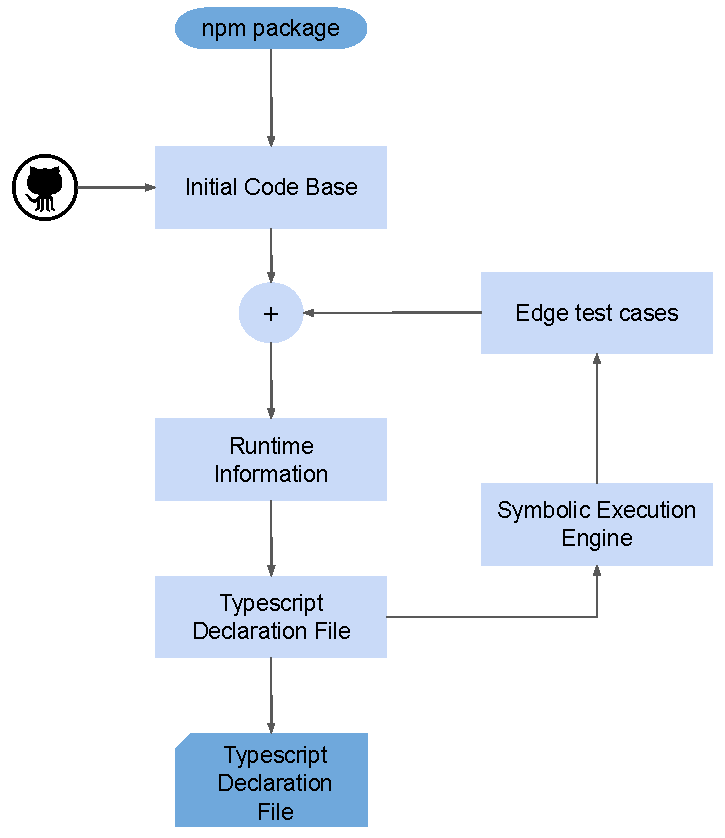
\includegraphics[width=0.9\textwidth]{figures/approach/typescript-declaration-files-generation-method/typescript_declaration_files_generation_method_block_diagram.pdf}}
    \caption[TypeScript Declaration Files Generation Method]{\textbf{TypeScript Declaration Files Generation Method} - Initial code base is retrieved from the npm package's repository. A valid TypeScript Declaration File is generated using run-time information. A Symbolic Execution Engine creates test cases based on the generated Declaration File and via a feedback loop enriches the code base until the stopping criteria is reached. The final TypeScript Declaration File gets returned.}
    \label{fig:tsd_generation_method_block_diagram}
\end{centering}
\end{figure}


The method consists of a continuous refinement process. It generates a TypeScript Declaration File based on data flow and type information gathered at run-time from a code base that executes the JavaScript Library. The code base is expanded by a Symbolic Execution Engine that generates test cases using the generated type definitions. As a result, new execution paths are explored, gathering new run-time information and thus refining the declaration file in every iteration.

Following the goal of easing and automating the generation of TypeScript Declaration Files for existing JavaScript libraries, the method receives the name of the JavaScript Library published to the NPM Registry as an input argument and returns the corresponding TypeScript declaration file.

The declaration file returned by the method is valid and fully functional, making it suitable for being used within the development process. It contains no errors and matches the structure of the JavaScript Library under analysis, so that the JavaScript code generated after compilation runs. The conducted experiments included tests that consisted on replacing a specific type definition from DefinitelyTyped \citep{definitely-typed-repository} with the one generated in the experiments: TypeScript compilation was successful, the generated JavaScript code ran without errors and code intelligence features performed by IDEs like code completion worked as expected.

The feedback loop was not included in the implementation, though. As explained, exploring new execution paths by creating new test cases will refine the declaration files: new types will be assigned to different variables, new interfaces will be detected and existing interfaces will be defined more accurately by detecting new properties. From an incremental point of view, generating the declaration files from run-time information has to be developed in a first place. A declaration file must exist first so that it can be refined afterwards.

For that reason, the decision was to keep the focus on building an end-to-end architecture that supports the generation of valid declaration files for a specific JavaScript Library. The proposed architecture supports a future addition of the refinement loop, without modifying the existing blocks. The Symbolic Execution Engine will expand the existing code base by generating new test cases. The actual generation of declaration files remains unmodified. 

\subsection{Implementation}
As explained before, the DefinitelyTyped Repository is the official repository for finding declaration files for existing JavaScript libraries. The \textit{TypeScript Declaration Files Generation Method} is intended to be used on existing, published npm packages. The generated output TypeScript declaration file is a valid file which can be used for development and uploaded to the DefinitelyTyped Repository.

Code examples that execute the JavaScript Library are needed to extract the run-time information via code instrumentation. It is achieved by retrieving the examples provided in the README files of the repositories of the different libraries. This is generally the place where developers explicitly show how to use their code. It showed to be an appropriate and pragmatic way of extracting the developer's intention and providing an useful initial code base with meaningful examples, thus avoiding a possible cold start problem. 

The examples and the code base of the library are instrumented with Jalangi \citep{DBLP:conf/sigsoft/SenKBG13}\citep{DBLP:conf/sigsoft/SenKBG13a} to gather data flow information and type information at runtime. Jalangi is a dynamic analysis configurable framework that provides several analysis modules that were extended as needed to retrieve the required run-time information, which is then saved to an output JSON file. This block is written in JavaScript and it runs in Node.js within a Docker container.

A second independent block uses the run-time information to generate a TypeScript Declaration File. It infers the overall structure of the JS Library, the interfaces and the types from the JSON file. This block is a Node.js application written in TypeScript that also runs within a Docker container.

The signatures obtained from the generated declaration file are used to generate pre and post conditions on a Symbolic Execution Engine in order to build different test cases that explore new execution paths. The code from the test cases is then added to the existing code base and the declaration file is generated again using an expanded code base.

Running the TypeScript Declaration File Generation Tool with the same run-time information as input will always produce the same result. If new execution paths are covered by the test cases, new run-time information will be gathered and the declaration file will change accordingly. In order to obtain a sound analysis, the feedback loop would be iterated until the generated declaration files in consecutive iterations do not differ. However, by trading soundness for scalability, the overall procedure can be stopped either using a loop bound, a time bound or an heuristics mechanism. 

The command line interface was inspired in the \mintinline{text}{dts-gen} \citep{dts-gen} package, a declaration files generator developed by Microsoft which is meant to be used as a starting point for writing declaration files. It can be seen in \coderef{code:dts-generate-example} that invoking the package is very simple and the only required argument is the name of the module published to the npm registry.

\begin{code}
  \begin{bashinline}
$ ./dts-generate abs
$ cat output/abs/index.d.ts 
export = Abs;

declare function Abs(input: string): string;

    \end{bashinline}
  \caption[Declaration file generation example]{\textbf{dts-generate usage} - Example of how to generate a declaration file for module \mintinline{text}{abs}.}
  \label{code:dts-generate-example}
\end{code}

\section{Initial code base} \label{sec:initial-code-base}
To extract run-time information of a JavaScript Library, it is necessary, by definition, to actually execute the code. It is not enough to instrument the source files of the library. The analysis modules provided by Jalangi to gather information are only triggered if the instrumented code gets executed.

It was decided to extract the code examples from the Readme files of the repository associated to the NPM Package. Readme files are usually used by developers for briefly describing what the code does, what problem it solves, how to install the application, how to build the code, etc. It is very common that developers provide code examples in the readme files to show how the code works and how to use it. This is specially true for NPM Packages, which are in general created to solve a specific problem of JavaScript development.

Obtaining code examples for a specific NPM Package is achieved in three steps:
\begin{enumerate}
  \item Obtaining the repository from the package.
  \item Retrieving the README file from the repository.
  \item Extract the code examples from the README file.
\end{enumerate}

\subsection{Repository}
The \mintinline{text}{npm view} command shows data about a package. It is possible to retrieve a specific field of the package registry by specifying the field name after the package descriptor. For example to retrieve information about the \mintinline{text}{lodash} package, the following command can be used: \mintinline{text}{npm view lodash}.

For this particular case, only the url of the repository associated with the package is needed. This can be achieved by adding the corresponding field name: \mintinline{text}{npm view <PACKAGE> repository.url}.

\begin{bashinline}
$ npm view npm repository.url
git+https://github.com/npm/cli.git

$ npm view lodash repository.url
git+https://github.com/lodash/lodash.git

$ npm view jquery repository.url$
git+https://github.com/jquery/jquery.git
\end{bashinline}

\subsection{Readme files}
The url for downloading a raw file from a Github Repository is the following:

\begin{bashinline}
https://raw.githubusercontent.com/THE-REPOSITORY/master/PATH-TO-FILE
\end{bashinline}

After the repository url is extracted from the npm package, the url for downloading the readme file needs to be constructed performing some string manipulation. Finally, the readme file is obtained with a simple \mintinline{text}{curl} or \mintinline{text}{wget} command.

\begin{bashinline}
$ npm view abs repository.url
git+ssh://git@github.com/IonicaBizau/abs.git

$ curl -L -o readme.md --fail \
    https://raw.githubusercontent.com/IonicaBizau/abs/master/README.md
\end{bashinline}

\subsection{Code examples}
Readme files are written using Markdown\footnote{https://www.markdownguide.org}, a very common lightweight and simple markup language. GitHub or BitBucket will convert the readme files into HTML automatically and render them when accessing the repository through a web browser.

It is very common to write code examples within code blocks indicating the programming language, so that it gets highlighted with the specific syntax. The Markdown identifiers for JavaScript are \mintinline{text}{js} or \mintinline{text}{javascript}. The code examples are finally retrieved by filtering the content within the corresponding code blocks.

\begin{textinline}
$ cat example-readme.md
# Description
This is an example that shows how to use console.log().

```js
var a = "Hello World!";

function f(s) {
	console.log(s);
}

f(a);
```

$ cat example-readme.md | \
  sed 's/```javascript/```js/g' | \
  sed -n '/^```js/,/^```/ p' > example.js

$ node example.js
Hello World!
\end{textinline}

\section{Run-time Information Gathering} \label{run-time-information-gathering}
As shown in a simple example in \figref{fig:run-time-information-gathering-simple-example}, run-time analysis will gather information such as:

\begin{enumerate}
  \item Function \mintinline{text}{f} got invoked with parameters \mintinline{text}{a} and \mintinline{text}{b} with types \mintinline{text}{string} and \mintinline{text}{number}.
  \item Property or method \mintinline{text}{foo} of parameter \mintinline{text}{a} of function \mintinline{text}{f} was accessed within the function.
  \item Parameter \mintinline{text}{a} of function \mintinline{text}{f} was used as operand for operator \mintinline{text}{==}.
\end{enumerate}

The dynamic analysis framework used for gathering this kind of information is Jalangi. As explained in \secref{sec:jalangi}, the configurable analysis modules enable programming custom callbacks that get triggered with virtually any JavaScript event. The events that are observed are:
\begin{enumerate}
  \item Binary operations, like \mintinline{text}{==}, \mintinline{text}{+} or \mintinline{text}{===}.
  \item Variable declaration.
  \item Function, method, or constructor invocation.
  \item Access to an object's property.
  \item Unary operations, like \mintinline{text}{!} or \mintinline{text}{typeof}.
\end{enumerate}

The implementation stores these observations as entities called \textit{interactions}. As explained later in \secref{sec:run-time-analysis}, they are used for translating, modifying and aggregating Jalangi's raw event information in order to get an application specific data representation.

The main goal of the run-time analysis is to gather information useful for determining a function's signature. Therefore, observations need to get associated with a function's argument. The implementation wraps variables around Proxy Objects to store tracking data, hereby enabling to associate the observation with a specific argument. The effect is reverted using Jalangi's callbacks to modify the behavior of the affected operators, such as \mintinline{text}{===} or \mintinline{text}{typeof}.

Jalangi fails to instrument some JavaScript libraries. No effort was made in trying to fix failing instrumentation. Failing JS libraries were omitted from the analysis by providing a list with the names of the modules that should not be instrumented.

Each function is given an unique key, which is used as the primary key of a map where the run-time information is stored. Each function has an array of arguments and each interaction gets associated with an argument. The map is finally returned as a JSON file that can be used for later processing.

The tool is written in JavaScript and runs in Node.js within a Docker container.

\begin{figure}[tp]
	\centering
	\begin{lrbox}{\mintedbox}
		\begin{minipage}{0.4\textwidth}
			\jscode{code/run-time-information-gathering/simple-examples/simple-example.js}
		\end{minipage}
	\end{lrbox}
	\subfloat[Instrumented JS code]{\usebox{\mintedbox}}
	\hfill
	\begin{lrbox}{\mintedbox}
		\begin{minipage}{0.58\textwidth}
			\jsoncode{code/run-time-information-gathering/simple-examples/output-simple-example.json}
		\end{minipage}
	\end{lrbox}
	\subfloat[Run-time information output]{\usebox{\mintedbox}}
	\caption[Simple run-time information gathering example]{\textbf{Simple run-time information gathering example} - Example code showing \textit{inputValue} and \textit{getField} interactions. Several additional fields and entries of the final output JSON file were omitted for simplicity.}
	\label{fig:run-time-information-gathering-simple-example}
\end{figure}

\subsection{Analysis} \label{sec:run-time-analysis}
The provided analysis module implements the following Jalangi callbacks, which were explained in detail in \secref{sec:jalangi}:
\begin{itemize}
  \item binaryPre()
  \item declare()
  \item getFieldPre()
  \item setFieldPre()
  \item functionEnter()
  \item functionExit()
  \item invokeFun()
  \item invokeFunPre()
  \item unaryPre()
  \item write()
\end{itemize}

They enable observation of all JS operations considered relevant. Every invoked function is given an unique identifier and information for each argument of every function gets stored. The entities \mintinline{text}{FunctionContainer}, \mintinline{text}{ArgumentContainer} and \mintinline{text}{Interaction} are introduced to support the representation of the gathered run-time information. 

Run-time information is stored in a map that contains objects of type \mintinline{text}{FunctionContainer}.
This entity contains static information about the function as well as implementation specific data needed for generating the right type of declaration file, as explained in \secref{sec:declaration-files-background}. Each field of the entity is explained in \coderef{code:function-container}.

\begin{code}
  \jscode{code/run-time-information-gathering/analysis/function-container.js}
  \caption[FunctionContainer object]{\textbf{\mintinline{text}{FunctionContainer} object} - \mintinline{text}{FunctionContainer} is the main entity in the map where the run-time information gets gathered. It contains implementation specific information for the declaration files generation. Entities of type \mintinline{text}{ArgumentContainer} get appended to the \mintinline{text}{args} property.}
  \label{code:function-container}
\end{code}

Moreover, as explained in \coderef{code:argument-container}, the \mintinline{text}{ArgumentContainer} object works as a container for all interactions recorded for that argument. Additionally, it contains simple information about the argument itself, like the index or the name given in the function declaration.

\begin{code}
  \jscode{code/run-time-information-gathering/analysis/argument-container.js}
  \caption[ArgumentContainer object]{\textbf{\mintinline{text}{ArgumentContainer} object} - The \mintinline{text}{ArgumentContainer} object works mainly as a container for all relevant observations regarding that argument.}
  \label{code:argument-container}
\end{code}

Finally, observations on the arguments of a function are stored as objects of type \mintinline{text}{Interaction}. They have to be always associated to an \mintinline{text}{ArgumentContainer} object or to another \mintinline{text}{Interaction}. They are explained in detail in \secref{sec:run-time-interactions}.

\subsection{Interactions} \label{sec:run-time-interactions}
Jalangi enables the developer to create custom analysis modules by implementing the callbacks that are relevant for the application. However, the callbacks belong to an abstraction layer that is not aware of the actual implementation. 

Observations of the arguments are stored as \mintinline{text}{Interactions}. They represent the relevant observation data that needs to be extracted for the purpose of best describing a function in order to generate a TypeScript declaration file.

The object \mintinline{text}{Interaction} is associated to an \mintinline{text}{ArgumentContainer}. If the \mintinline{text}{ArgumentContainer} does not exist when the Jalangi callback is triggered, the \mintinline{text}{Interaction} is not saved. The main goal of gathering run-time information is to describe a function and its arguments. Thus, callbacks triggered on variables that are not arguments of functions are ignored, as shown in \coderef{code:ignored-observations}. The mechanism to map an observation with an \textit{ArgumentContainer} is described in detail in \secref{sec:run-time-wrapper-objects}

\begin{code}
  \jscode{code/run-time-information-gathering/analysis/ignored-observations.js}
  \caption[Ignored observations]{\textbf{Ignored observations} - Variable \mintinline{text}{b} gets declared within the scope of function \mintinline{text}{foo}. Therefore, no observation on it gets stored.}
  \label{code:ignored-observations}
\end{code}

\subsubsection{\textit{inputValue} interaction}
It is the most simple interaction. As shown in \figref{fig:run-time-information-gathering-input-value}, it gets triggered when a function is invoked and it stores the input value of a specific argument. If a function gets invoked several times, different interactions get stored, each one of them with a different \mintinline{text}{traceId}.

\begin{figure}[tp]
	\centering
	\begin{lrbox}{\mintedbox}
		\begin{minipage}{0.4\textwidth}
			\jscode{code/run-time-information-gathering/simple-examples/input-value.js}
		\end{minipage}
	\end{lrbox}
	\subfloat[Instrumented JS code]{\usebox{\mintedbox}}
	\hfill
	\begin{lrbox}{\mintedbox}
		\begin{minipage}{0.58\textwidth}
			\jsoncode{code/run-time-information-gathering/simple-examples/output-input-value.json}
		\end{minipage}
	\end{lrbox}
	\subfloat[Run-time information output]{\usebox{\mintedbox}}
	\caption[\textit{inputValue} interaction example]{\textbf{\textit{inputValue} interaction example} - The type of the arguments of function \textit{foo()} is recorded. Several additional fields and entries of the final output JSON file were omitted for simplicity.}
	\label{fig:run-time-information-gathering-input-value}
\end{figure}

\subsubsection{\textit{getField} interaction}
This interaction gets triggered whenever a property of an object gets accessed, either if the get field operation is \mintinline{text}{obj.field} or \mintinline{text}{obj['field']}. As shown in \figref{fig:run-time-information-gathering-get-field}, the name of the accessed field and the type of the actual property get stored.

It should be noted that the field \mintinline{text}{returnTypeOf} represents the type of the accessed property at the time when the interaction gets triggered. The accessed property may somehow get modified afterwards, which will not modify the existing interaction. If the property gets accessed again, a new interaction with a new \mintinline{text}{returnTypeOf} value will be added, as shown in \coderef{code:get-field-changing-at-runtime}.

\begin{code}
  \jscode{code/run-time-information-gathering/analysis/get-field-changing-at-runtime.js}
  \caption[Modified accessed property]{\textbf{Modified accessed property} - Variable \mintinline{text}{b} gets declared within the scope of function \mintinline{text}{foo}. Therefore, no observation on it gets stored.}
  \label{code:get-field-changing-at-runtime}
\end{code}

\begin{figure}[tp]
	\centering
	\begin{lrbox}{\mintedbox}
		\begin{minipage}{0.4\textwidth}
			\jscode{code/run-time-information-gathering/simple-examples/get-field.js}
		\end{minipage}
	\end{lrbox}
	\subfloat[Instrumented JS code]{\usebox{\mintedbox}}
	\hfill
	\begin{lrbox}{\mintedbox}
		\begin{minipage}{0.58\textwidth}
			\jsoncode{code/run-time-information-gathering/simple-examples/output-get-field.json}
		\end{minipage}
	\end{lrbox}
	\subfloat[Run-time information output]{\usebox{\mintedbox}}
	\caption[\textit{getField} interaction example]{\textbf{\textit{getField} interaction example} - The accessed properties of argument \textit{a} with their type are recorded. Several additional fields and entries of the final output JSON file were omitted for simplicity.}
	\label{fig:run-time-information-gathering-get-field}
\end{figure}

\subsubsection{\textit{methodCall} interaction}
This interaction gets triggered with the invocation of an object's method. As explained in \figref{fig:run-time-information-gathering-method-call}, information about the method itself is stored as another \mintinline{text}{FunctionContainer} in the overall map. The reference to the \mintinline{text}{FunctionContainer} is achieved through the properties \mintinline{text}{functionId} and \mintinline{text}{traceIdInTargetFunction}.

\begin{figure}[h]
	\centering
	\begin{lrbox}{\mintedbox}
		\begin{minipage}{0.4\textwidth}
			\jscode{code/run-time-information-gathering/simple-examples/method-call.js}
		\end{minipage}
	\end{lrbox}
	\subfloat[Instrumented JS code]{\usebox{\mintedbox}}
	\hfill
	\begin{lrbox}{\mintedbox}
		\begin{minipage}{0.58\textwidth}
			\jsoncode{code/run-time-information-gathering/simple-examples/output-method-call.json}
		\end{minipage}
	\end{lrbox}
	\subfloat[Run-time information output]{\usebox{\mintedbox}}
	\caption[\textit{methodCall} interaction example]{\textbf{\textit{methodCall} interaction example} - The invoked method of argument \textit{a} is recorded. Method information can be accessed through the reference \mintinline{bash}{functionId}, for which, in this example, the \mintinline{bash}{inputValue} interactions are stored. Main entry for \mintinline{bash}{functionId_3} has been ommited. Several additional fields and entries of the final output JSON file were also ommited for simplicity.}
	\label{fig:run-time-information-gathering-method-call}
\end{figure}

\subsubsection{\textit{setField} interaction}
The trigger for this interaction is writing an object's property, either by accessing the field as \mintinline{text}{obj.field = 1} or \mintinline{text}{obj['field'] = 1}. It can be seen in \figref{fig:run-time-information-gathering-set-field} that the interaction contains the name of the property to be written and the type of the value to be stored.

\begin{figure}[tp]
	\centering
	\begin{lrbox}{\mintedbox}
		\begin{minipage}{0.4\textwidth}
			\jscode{code/run-time-information-gathering/simple-examples/set-field.js}
		\end{minipage}
	\end{lrbox}
	\subfloat[Instrumented JS code]{\usebox{\mintedbox}}
	\hfill
	\begin{lrbox}{\mintedbox}
		\begin{minipage}{0.58\textwidth}
			\jsoncode{code/run-time-information-gathering/simple-examples/output-set-field.json}
		\end{minipage}
	\end{lrbox}
	\subfloat[Run-time information output]{\usebox{\mintedbox}}
	\caption[\textit{setField} interaction example]{\textbf{\textit{setField} interaction example} - When a property of an argument gets written, the name of the written property and the type are recorded. Several additional fields and entries of the final output JSON file were also omitted for simplicity.}
	\label{fig:run-time-information-gathering-set-field}
\end{figure}


\subsubsection{\textit{usedAsArgument} interaction}
The run-time information is stored in a map with one \mintinline{text}{FunctionContainer} entry per function. As seen in \figref{fig:run-time-information-gathering-used-as-argument}, an argument of function \mintinline{text}{foo()} is used as parameter to invoke a second function \mintinline{text}{bar()}. Interactions triggered within function \mintinline{text}{bar()} are going to be stored within the \mintinline{text}{FunctionContainer} corresponding to function \mintinline{text}{bar()}, i.e. not the one associated to function \mintinline{text}{foo()}.

However, for the example provided in \figref{fig:run-time-information-gathering-used-as-argument} it is relevant to also associate interactions triggered within function \mintinline{text}{bar()} to the function \mintinline{text}{foo()}, since they can  be useful for describing the argument of \mintinline{text}{foo()} more accurately.

Therefore, \mintinline{text}{usedAsArgument} interaction is introduced. It gets triggered when an argument is used in the invocation of a consecutive function. It serves the purpose of connecting related interactions. As shown in \figref{fig:run-time-information-gathering-used-as-argument}, it mainly contains information for identifying the target \mintinline{text}{FunctionContainer}.

\begin{figure}[h]
	\centering
	\begin{lrbox}{\mintedbox}
		\begin{minipage}{0.3\textwidth}
			\jscode{code/run-time-information-gathering/simple-examples/used-as-argument.js}
		\end{minipage}
	\end{lrbox}
	\subfloat[Instrumented JS code]{\usebox{\mintedbox}}
	\hfill
	\begin{lrbox}{\mintedbox}
		\begin{minipage}{0.68\textwidth}
			\jsoncode{code/run-time-information-gathering/simple-examples/output-used-as-argument.json}
		\end{minipage}
	\end{lrbox}
	\subfloat[Run-time information output]{\usebox{\mintedbox}}
	\caption[\textit{usedAsArgument} interaction example]{\textbf{\textit{usedAsArgument} interaction example} - Reporting when an argument is used as an argument of another function provides more accurate information. Several additional fields and entries of the final output JSON file were ommited for simplicity.}
	\label{fig:run-time-information-gathering-used-as-argument}
\end{figure}

\subsubsection{\textit{operator} interaction}
Identifying if an argument is used with a specific operator is very important for inferring the type of that variable. Relational operators like \mintinline{text}{<, >, <=, >=} are mainly used with type \mintinline{text}{number}. On the other side, operator \mintinline{text}{+} is mainly used with \mintinline{text}{number} or \mintinline{text}{string}. Empirical evidence of how operators are used is presented in \secref{sec:experiments-js-operators-usage}.

The \mintinline{text}{operator} interaction stores the operator being used and the type of the left hand and right hand operands. It also indicates which operand is the one that triggered the interaction. \figref{fig:run-time-information-gathering-operator} provides an example for operator \mintinline{text}{+}.

The supported operators are the ones that trigger Jalangi's \mintinline{text}{binaryPre()} callback. Conditionals are merged into one operator name \mintinline{text}{conditional}, since Jalangi's \mintinline{text}{conditional()} callback does not offer a way of identifying the operator for this cases. Both callbacks are explained in section \secref{sec:jalangi}. Right hand operand is left as \mintinline{text}{undefined} for that case.

\begin{figure}[h]
	\centering
	\begin{lrbox}{\mintedbox}
		\begin{minipage}{0.34\textwidth}
			\jscode{code/run-time-information-gathering/simple-examples/operator.js}
		\end{minipage}
	\end{lrbox}
	\subfloat[Instrumented JS code]{\usebox{\mintedbox}}
	\hfill
	\begin{lrbox}{\mintedbox}
		\begin{minipage}{0.62\textwidth}
			\jsoncode{code/run-time-information-gathering/simple-examples/output-operator.json}
		\end{minipage}
	\end{lrbox}
	\subfloat[Run-time information output]{\usebox{\mintedbox}}
	\caption[\textit{operator} interaction example]{\textbf{\textit{operator} interaction example} - The interaction records the operator and the type of both operands. The field \mintinline{bash}{operandForInteraction} indicates which operand triggered the interaction. The example shows how that value is \mintinline{bash}{left} for one argument and \mintinline{bash}{right} for the other one. Several additional fields and entries of the final output JSON file were ommited for simplicity.}
	\label{fig:run-time-information-gathering-operator}
\end{figure}

\subsubsection{\textit{followingInteractions}}
If a property of an argument is accessed the Jalangi callback \mintinline{text}{getField()} gets triggered and a \mintinline{text}{getField} interaction gets associated to the corresponding \mintinline{text}{ArgumentContainer}. In order to describe the interface of the argument more accurately, it is also relevant to recursively record if properties of the return values are accessed, as explained in \figref{fig:run-time-information-gathering-following-interactions}.

This was implemented by not only mapping the observation with an \mintinline{text}{ArgumentContainer} but also with a \mintinline{text}{getField} or \mintinline{text}{methodCall} interaction. Both \mintinline{text}{ArgumentContainer} and \mintinline{text}{Interaction} implement the \mintinline[breaklines]{javascript}{addInteraction} method, as shown in \coderef{code:add-interaction-example}

\begin{code}
  \jscode{code/run-time-information-gathering/analysis/add-interaction-example.js}
  \caption[addInteraction method]{\textbf{addInteraction method} - Example showing how interactions can be associated with \mintinline{text}{ArgumentContainer} or with another \mintinline{text}{Interaction}.}
  \label{code:add-interaction-example}
\end{code}

\begin{figure}[tp]
	\centering
	\begin{lrbox}{\mintedbox}
		\begin{minipage}{0.4\textwidth}
			\jscode{code/run-time-information-gathering/simple-examples/following-interactions.js}
		\end{minipage}
	\end{lrbox}
	\subfloat[Instrumented JS code]{\usebox{\mintedbox}}
	\hfill
	\begin{lrbox}{\mintedbox}
		\begin{minipage}{0.58\textwidth}
			\jsoncode{code/run-time-information-gathering/simple-examples/output-following-interactions.json}
		\end{minipage}
	\end{lrbox}
	\subfloat[Run-time information output]{\usebox{\mintedbox}}
	\caption[\textit{followingInteractions} interaction example]{\textbf{\textit{followingInteractions} interaction example} - Observations on return values of \mintinline{bash}{getField} and \mintinline{bash}{methodCall} interactions get associated to the leading interaction. Several additional fields and entries of the final output JSON file were omitted for simplicity.}
	\label{fig:run-time-information-gathering-following-interactions}
\end{figure}

\subsubsection{Traces}
Different executions of a function are identified through different \mintinline{text}{traceIds}. Each interaction and return value of a \mintinline{text}{FunctionContainer} stores the corresponding \mintinline{text}{traceId}. The \mintinline{text}{traceId} field enables identifying correlations between input types and return values. An example is provided in \figref{fig:run-time-information-gathering-traces}. The field can also be helpful in determining common interactions happening on the same execution path.

\begin{figure}[tp]
	\centering
	\begin{lrbox}{\mintedbox}
		\begin{minipage}{0.46\textwidth}
			\jscode{code/run-time-information-gathering/simple-examples/traces.js}
		\end{minipage}
	\end{lrbox}
	\subfloat[Instrumented JS code]{\usebox{\mintedbox}}
	\hfill
	\begin{lrbox}{\mintedbox}
		\begin{minipage}{0.52\textwidth}
			\jsoncode{code/run-time-information-gathering/simple-examples/output-traces.json}
		\end{minipage}
	\end{lrbox}
	\subfloat[Run-time information output]{\usebox{\mintedbox}}
	\caption[\textit{traces} example]{\textbf{\textit{traces} example} - Interactions on different invocations of a function are stored with different \mintinline{bash}{traces}. Several additional fields and entries of the final output JSON file were omitted for simplicity.}
	\label{fig:run-time-information-gathering-traces}
\end{figure}


\subsection{Wrapper Objects} \label{sec:run-time-wrapper-objects}
An \mintinline{text}{Interaction} needs to be associated to an \mintinline{text}{ArgumentContainer} or to another \mintinline{text}{Interaction}. This means that when Jalangi triggers a callback, it must be determined if that callback is relevant or not, i.e. if that callback refers to an argument of an invoked function. However, this can not be determined by only using the information provided in the different callbacks.

However, Jalangi exposes the actual value affected by the callback. For example, for the \mintinline{text}{getField()} callback triggered by operation \mintinline{javascript}{myObj.prop}, Jalangi does provide the object \mintinline{javascript}{myObj} in the callback.

The solution consists in wrapping every input argument around a Wrapper Object when the function gets invoked. The Wrapper Object will store the reference to the corresponding \mintinline{text}{ArgumentContainer} or \mintinline{text}{Interaction}. Jalangi callbacks will then get triggered on the Wrapper Object instead. A mapping with the corresponding \mintinline{text}{ArgumentContainer} or \mintinline{text}{Interaction} is then straightforward, since the reference can be directly retrieved from the Wrapper Object.

Jalangi enables to modify the behavior of the original code. Using \mintinline{text}{invokFunPre} and \mintinline{javascript}{declare} callbacks, a function invocation is detected and the arguments of the function are modified in run-time.

Every function invocation generates new Wrapper Objects, which means that a Wrapper Object represents the input argument for a specific invocation. \mintinline{text}{TraceIds} are also stored within these objects.

The solution extends a similar concept already implemented by Jalangi: \mintinline{text}{ShadowObjects}. It is a unique object associated to another object which can store meta-information. However, a \mintinline{text}{ShadowObject} can not be created for primitives values, which is a major drawback. It is indeed relevant to capture, for example, if a \mintinline{text}{number} is being used with a particular operator or if the property \mintinline{text}{length} of a \mintinline{text}{string} is being accessed.

The implemented solution wraps objects around JavaScript Proxies. Primitive values like \mintinline{text}{number} or \mintinline{text}{string} are converted to their native wrapper objects, i.e. \mintinline{text}{Number} and \mintinline{text}{String}. Finally, \mintinline{text}{null} and \mintinline{text}{undefined} are converted to empty objects with modified \mintinline{text}{valueOf()} and \mintinline{text}{toString()} methods.

The behavior of the original code is being explicitly modified. Therefore, original values are used instead for affected operators like \mintinline{text}{===, !==, typeof}, for which wrapper objects will not work as expected. For \mintinline{text}{null} and \mintinline{text}{undefined} wrappers, the original values are used for conditional operators, since the result of the abstract operation \mintinline{text}{ToBoolean} on an object is always \mintinline{text}{true}, as defined in the ECMAScript Language Specification \citep{ecma-script}. This approach could have been used for every operation by using the original value in the affected Jalangi callbacks. However, the implementation is complex and error prone. Instead, it was decided to modify the corresponding methods or specific operators so that they are compliant with JavaScript Type Coercion, which is explained in detail in {sec:background-js-type-coercion}.

\subsection{Output}
Information is stored in a map containing \mintinline{text}{FunctionContainer} entries. When the executions stops, Jalangi's callback \mintinline{text}{endExecution()} is called and the information is saved as a JSON to a file.


\subsection{Blacklisted Modules}
When instrumenting a JS Library, Jalangi will try to instrument all required modules by resolving and finding the modules. Unfortunately, Jalangi's native behavior is to stop the complete analysis if there is an error in the instrumentation of any of the required modules or in the script itself.

The workaround introduced by the implementation modifies Jalangi's behavior for failing instrumentation. For a given required module, it first tries to instrument it. If the instrumentation if unsuccessful, it simply skips the instrumentation and returns the original module without instrumenting it.

As expected, no Jalangi callbacks will be triggered for that module's code. However, this workaround enables to at least still get run-time information of other required modules by not breaking the complete analysis. As explained in \figref{fig:blacklisted-modules}, instead of stopping the analysis, failing modules are skipped but modules required by them do get instrumented anyway. Modifying Jalangi's instrumentation algorithm is out of the scope of this work.

The application can be invoked by passing an optional argument with the path to a a JSON file containing the list of modules that should not be instrumented.

\begin{figure}[tp]
	\centering
	\begin{lrbox}{\mintedbox}
		\begin{minipage}{0.45\textwidth}
			\jscode{code/blacklisted-modules/foo.js}
		\end{minipage}
	\end{lrbox}
	\subfloat[foo/index.js]{\usebox{\mintedbox}}
	\hfill
	\begin{lrbox}{\mintedbox}
		\begin{minipage}{0.45\textwidth}
			\jscode{code/blacklisted-modules/A.js}
		\end{minipage}
	\end{lrbox}
	\subfloat[A/index.js]{\usebox{\mintedbox}}

	\begin{lrbox}{\mintedbox}
		\begin{minipage}{0.48\textwidth}
			\jscode{code/blacklisted-modules/D.js}
		\end{minipage}
	\end{lrbox}
	\subfloat[D/index.js]{\usebox{\mintedbox}}
	\hfill
	\begin{lrbox}{\mintedbox}
		\begin{minipage}{0.45\textwidth}
			\jsoncode{code/blacklisted-modules/blacklist.json}
		\end{minipage}
	\end{lrbox}
	\subfloat[blacklist.json]{\usebox{\mintedbox}}

	\subfloat{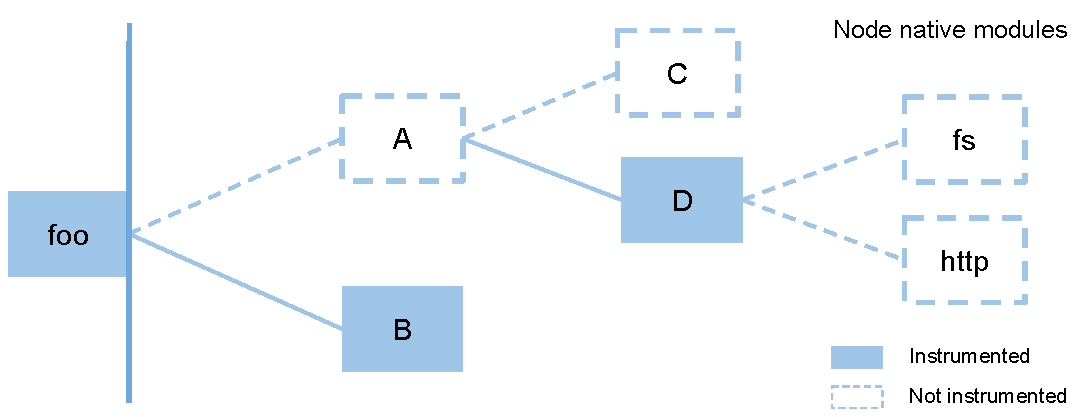
\includegraphics[width=1\textwidth]{figures/approach/blacklisted-modules/blacklisted-modules.pdf}}
	
	\caption[Non-instrumented node modules]{\textbf{Non-instrumented node modules} - Dependencies tree for module \textit{foo}. Modules \textit{A} and \textit{B} are included in the blacklist. Module \textit{D} is instrumented anyway, even though its parent is not. Node native modules, like \textit{fs} or \textit{http}, are excluded anyway by Jalangi.}
	\label{fig:blacklisted-modules}
\end{figure}

\section{TypeScript Declaration File Generation}
The actual generation of the declaration file is the next step in the pipeline after gathering the run-time information, as shown in \figref{fig:tsd_generation_method_block_diagram}. It is a lightweight, simple and fast application, which does not interact with the actual JavaScript module at run-time. Instead, it uses the JSON output file containing the run-time information and generates a TypeScript declaration file which is use ready to be used within a TypeScript project. The tool itself is written in TypeScript and runs within a Docker container in NodeJS. 

\subsection{Templates}
TypeScript provides templates for writing declaration files, as explained in \secref{sec:declaration-files-background}. Each template corresponds to a different way of exporting a JS module. The code uses different fields from the \mintinline{text}{FunctionContainer} entity in the run-time information to detect how the module is being used:

\begin{itemize}
  \item \mintinline{text}{requiredModule}: The name of the module that exported the corresponding function. It is useful for processing only functions exported by the module for which the declaration files is being generated.
  \item \mintinline{text}{isExported}: Boolean that indicates whether the function is exported when importing the module.
  \item \mintinline{text}{isConstructor}: Boolean that indicates whether the function was used as a constructor through the \mintinline{text}{new} operator.
  \item \mintinline{text}{constructedBy}: Indicates the \mintinline{text}{functionId} that constructed the object invoking the corresponding function.
\end{itemize}

The following templates were implemented:

\begin{enumerate}
  \item \mintinline{text}{module.d.ts}: The code checks if the exported module is neither a function nor a constructor, i.e. if properties \mintinline{text}{isExported} and \mintinline{text}{isConstructor} are \mintinline{text}{false}. An example is provided in \figref{fig:ts-declaration-file-module-template}.

  \item \mintinline{text}{module-class.d.ts}: The code will use this template when both the fields \mintinline{text}{isExported} and \mintinline{text}{isConstructor} are true. It should be noted that the module exports only the constructor function. Methods belonging to the class are detected using the \mintinline{text}{constructedBy} field from the run-time data.
  
  \item \mintinline{text}{module-function.d.ts}: The field \mintinline{text}{isExported} field is used to determine whether this templates should be used or not. An example is provided in \figref{fig:ts-declaration-file-module-function-template}. If further interfaces or types are required, they are written within a namespace named like the exported function.
\end{enumerate}

\begin{figure}[h]
	\centering
	\begin{lrbox}{\mintedbox}
		\begin{minipage}{0.7\textwidth}
			\jscode{code/typescript-declaration-file-generation/templates/module/index.js}
		\end{minipage}
	\end{lrbox}
	\subfloat[index.js - Entry point to be executed with \mintinline{bash}{node index.js}]{\usebox{\mintedbox}}
	
	\begin{lrbox}{\mintedbox}
		\begin{minipage}{0.7\textwidth}
			\jscode{code/typescript-declaration-file-generation/templates/module/calculator.js}
		\end{minipage}
	\end{lrbox}
	\subfloat[calculator.js - Module for which the TS Declaration File is going to be generated]{\usebox{\mintedbox}}

	\begin{lrbox}{\mintedbox}
		\begin{minipage}{0.9\textwidth}
			\tscode{code/typescript-declaration-file-generation/templates/module/index.d.ts}
		\end{minipage}
	\end{lrbox}
	\subfloat[calculator/index.d.ts]{\usebox{\mintedbox}}

	\caption[module.d.ts template example]{\textbf{module.d.ts template example} - Declaration file for the \mintinline{bash}{calculator} module is generated using the \mintinline{bash}{module.d.ts} template.}
	\label{fig:ts-declaration-file-module-template}
\end{figure}

\begin{figure}[h]
	\centering
	\begin{lrbox}{\mintedbox}
		\begin{minipage}{0.48\textwidth}
			\jscode{code/typescript-declaration-file-generation/templates/module-class/index.js}
		\end{minipage}
	\end{lrbox}
	\subfloat[index.js - Entry point to be executed with \mintinline{bash}{node index.js}]{\usebox{\mintedbox}}
	\hfill
	\begin{lrbox}{\mintedbox}
		\begin{minipage}{0.5\textwidth}
			\jscode{code/typescript-declaration-file-generation/templates/module-class/calculator.js}
		\end{minipage}
	\end{lrbox}
	\subfloat[calculator.js - Module for which the TS Declaration File is going to be generated]{\usebox{\mintedbox}}

	\begin{lrbox}{\mintedbox}
		\begin{minipage}{0.7\textwidth}
			\tscode{code/typescript-declaration-file-generation/templates/module-class/calculator.d.ts}
		\end{minipage}
	\end{lrbox}
	\subfloat[calculator/index.d.ts]{\usebox{\mintedbox}}

	\begin{lrbox}{\mintedbox}
		\begin{minipage}{0.7\textwidth}
			\tscode{code/typescript-declaration-file-generation/templates/module-class/index.ts}
		\end{minipage}
	\end{lrbox}
	\subfloat[index.ts - TypeScript file using the generated declaration file]{\usebox{\mintedbox}}
	\caption[module-class.d.ts template example]{\textbf{module-class.d.ts template example} - Declaration file for the \mintinline{bash}{calculator} module is generated using the \mintinline{bash}{module-class.d.ts} template. Exported module can be used as a constructor within a TypeScript project.}
	\label{fig:ts-declaration-file-module-class-template}
\end{figure}

\begin{figure}[tp]
	\centering
	\begin{lrbox}{\mintedbox}
		\begin{minipage}{0.9\textwidth}
			\jscode{code/typescript-declaration-file-generation/templates/module-function/index.js}
		\end{minipage}
	\end{lrbox}
	\subfloat[index.js - Entry point to be executed with \mintinline{bash}{node index.js}]{\usebox{\mintedbox}}
	
	\begin{lrbox}{\mintedbox}
		\begin{minipage}{0.9\textwidth}
			\jscode{code/typescript-declaration-file-generation/templates/module-function/snake-to-camel.js}
		\end{minipage}
	\end{lrbox}
	\subfloat[snake-to-camel.js - Module for which the TS Declaration File is going to be generated]{\usebox{\mintedbox}}

	\begin{lrbox}{\mintedbox}
		\begin{minipage}{0.8\textwidth}
			\tscode{code/typescript-declaration-file-generation/templates/module-function/index.d.ts}
		\end{minipage}
	\end{lrbox}
	\subfloat[snake-to-camel/index.d.ts]{\usebox{\mintedbox}}

	\caption[module-function.d.ts template example]{\textbf{module-function.d.ts template example} - Declaration file for the \mintinline{bash}{snake-to-camel} module is generated using the \mintinline{bash}{module-function.d.ts} template.}
	\label{fig:ts-declaration-file-module-function-template}
\end{figure}

JavaScript constructors where explained in \secref{sec:background-javascript}. There are built-in functions that are not able to be used as a constructors. For example, if \mintinline{text}{Math} is intended to be used as a constructor with the \mintinline{text}{new} operator, the following error will arise: \mintinline{text}{TypeError: Math is not a constructor}. ES6 arrow functions are not allowed to used as a constructor either. However, for those functions that can be both used as constructors or called as regular functions, there is no difference between them that actually indicate whether a function is intended to be used with the \mintinline{text}{new} operator or not. The choice of using the \mintinline{text}{module-function.d.ts} or the \mintinline{text}{module-class.d.ts} template is made after executing the code and depends on how the function was used.

\coderef{code:typescript-templates-function-as-constructor} exposes a scenario for which a module could be inferred as \mintinline{text}{module-function.d.ts} or \mintinline{text}{module-class.d.ts} depending only on how it was executed. Thus, examples that execute the module under analysis by truly representing the developer's intention are crucial for an accurate generation of declaration files and inference of types and interfaces. As explained in \secref{sec:initial-code-base}, this was achieved by extracting the code examples written by the developers from the repositories.

\begin{code}
  \jscode{code/typescript-declaration-file-generation/templates/function-as-constructor.js}
  \caption[Choice between module-function.d.ts or module-class.d.ts]{\textbf{Choice between module-function.d.ts or module-class.d.ts} - If the exported module is used without the \mintinline{text}{new} operator, the \mintinline{text}{module-function.d.ts} template will be used. If used with the \mintinline{text}{new} operator, the \mintinline{text}{module-class.d.ts} template will be applied.}
  \label{code:typescript-templates-function-as-constructor}
\end{code}

\subsection{Interfaces}
Interfaces are created by exploring \mintinline{text}{getField} and \mintinline{text}{methodCall} interactions from the run-time information. The code will gather the interactions for a specific argument and build the interface by incrementally adding new properties. Interactions within the \mintinline{text}{followingInteractions} field are recursively traversed, building a new interface in each recursion level.

An example is provided in \figref{fig:ts-declaration-file-generation-interfaces}. The name given to the interface is based on the name of the input argument.

It can be also seen in \figref{fig:ts-declaration-file-generation-nested-interfaces} that nested interfaces are declared as independent interfaces and then declared as types of the prior interface.

\begin{figure}[h]
	\centering
	\begin{lrbox}{\mintedbox}
		\begin{minipage}{0.45\textwidth}
			\jscode{code/typescript-declaration-file-generation/example-with-interfaces/index.js}
		\end{minipage}
	\end{lrbox}
	\subfloat[index.js - Entry point to be executed with \mintinline{bash}{node index.js}]{\usebox{\mintedbox}}
	\hfill
	\begin{lrbox}{\mintedbox}
		\begin{minipage}{0.54\textwidth}
			\jscode{code/typescript-declaration-file-generation/example-with-interfaces/printer.js}
		\end{minipage}
	\end{lrbox}
	\subfloat[printer.js - Module for which the TS Declaration File is going to be generated]{\usebox{\mintedbox}}

	\begin{lrbox}{\mintedbox}
		\begin{minipage}{0.51\textwidth}
			\tscode{code/typescript-declaration-file-generation/example-with-interfaces/printer.d.ts}
		\end{minipage}
	\end{lrbox}
	\subfloat[printer/index.d.ts]{\usebox{\mintedbox}}
	\hfill
	\begin{lrbox}{\mintedbox}
		\begin{minipage}{0.48\textwidth}
			\tscode{code/typescript-declaration-file-generation/example-with-interfaces/index.ts}
		\end{minipage}
	\end{lrbox}
	\subfloat[index.ts]{\usebox{\mintedbox}}

	\caption[Interfaces inference]{\textbf{Interfaces inference} - Declaration file for the \mintinline{bash}{printer} module is generated using the \mintinline{bash}{module-function-d-ts} template. Interface of the input argument is generated correctly. The name of the interface is always generated as \mintinline{bash}{'I__ + argumentName'}, in this case \mintinline{bash}{I__input}.}
	\label{fig:run-time-information-gathering-get-field}
\end{figure}

\begin{figure}[tp]
	\centering
	\begin{lrbox}{\mintedbox}
		\begin{minipage}{0.7\textwidth}
			\jscode{code/typescript-declaration-file-generation/example-with-nested-interfaces/printer.js}
		\end{minipage}
	\end{lrbox}
	\subfloat[printer.js]{\usebox{\mintedbox}}

	\begin{lrbox}{\mintedbox}
		\begin{minipage}{0.9\textwidth}
			\tscode{code/typescript-declaration-file-generation/example-with-nested-interfaces/printer.d.ts}
		\end{minipage}
	\end{lrbox}
	\subfloat[printer/index.d.ts]{\usebox{\mintedbox}}

	\caption[Nested interfaces]{\textbf{Nested interfaces} - Sub-interfaces for fields \mintinline{bash}{name} and \mintinline{bash}{address} are declared as separated interfaces and then associated to the main \mintinline{bash}{I__employee} interface.}
	\label{fig:ts-declaration-file-generation-nested-interfaces}
\end{figure}

\subsection{Implementation}
The application runs within a Docker container. \coderef{code:declaration-file-generation-docker} explains how to build and run the application and how to extract the declaration file from the container.

\begin{code}
\begin{bashinline}
$ ./build/build.sh
$ docker run --name generate-declaration-file \
  -v PATH_TO_RUN_TIME_INFORMATION_JSON:/tmp/output.json \
  tsd-generator \
  --module-name calculator \
  -i /tmp/output.json

$ docker cp generate-declaration-file:/usr/local/app/output/. /tmp/ts-declaration-file
$ docker rm generate-declaration-file
$ cat /tmp/ts-declaration-file/calculator/index.d.ts
export function sum(a: number, b: number): number;
export function multiply(a: number, b: number): number;
\end{bashinline}
  \caption[Declaration file generation]{\textbf{Declaration file generation} - The Docker image needs to be built after cloning the repository. Afterwards, the declaration file is generated by the run-time information and then retrieved from the container.}
  \label{code:declaration-file-generation-docker}
\end{code}

\section{Evaluation}
After generating a declaration file for a published NPM module, it is necessary to evaluate the quality of it. It was decided to compare the generated declaration file against the one uploaded to the DefinitelyTyped repository for the same module, as shown in \figref{fig:evaluation-diagram}.

It is arguable, however, to use a baseline for evaluation that it is known to be incorrect or inaccurate for some modules. It was exposed in \secref{sec:problem-definition} that mismatches between definition files and JS libraries do exist. The presented approach actually tackles that issue. 

Nevertheless, it was decided that during a first stage of development comparing against DefinitelyTyped provides an acceptable baseline, guiding the tool to generate declaration files that are \textit{as good as} the ones uploaded to the repository. Furthermore, comparing two files is extremely fast, which is useful for creating an automated test suite that aids the development process.

Finally, in a future stage, declaration files should be checked against the JS library itself. Approaches based on feedback-directed random testing like TSTest already made considerable progress and new solutions could be built on top of them \citep{DBLP:journals/pacmpl/KristensenM17}.

\begin{figure}[h]
\begin{centering}
    {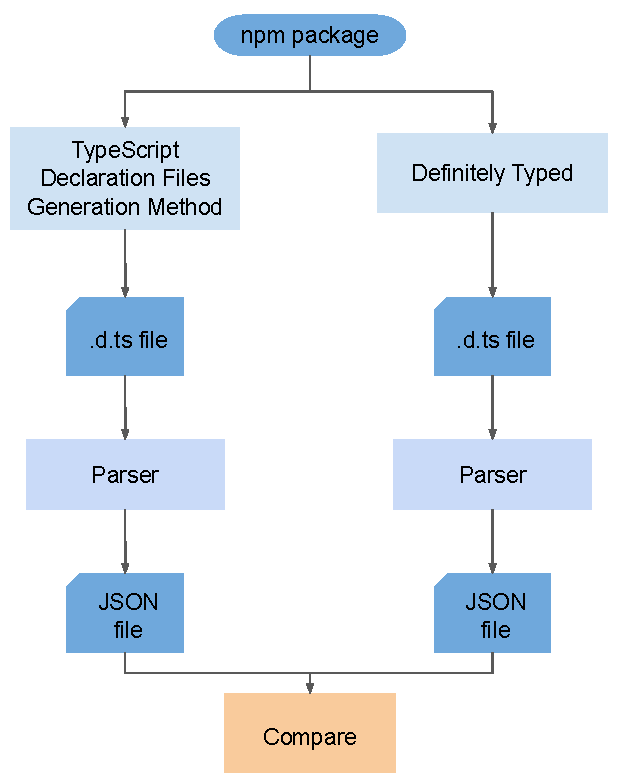
\includegraphics[width=0.8\textwidth]{figures/approach/evaluation/evaluation-diagram.pdf}}
    \caption[Evaluation against DefinitelyTyped Repository]{\textbf{Evaluation of generated declaration files against DefinitelyTyped Repository} - A parser transforms the generated declaration file and the equivalent file in the DefinitelyTyped repository into a JSON file using the TypeScript Compiler API \citep{typescript-compiler-api}. Comparison is then performed on the JSON files, i.e. not on the declaration files.}
    \label{fig:evaluation-diagram}
\end{centering}
\end{figure}


\subsection{Parsing} \label{sec:approach-parsing}
Before comparison, declaration files need to be parsed so that both of them share the same structure. It was achieved by using the TypeScript Compiler API, a library developed by Microsoft that allows to traverse the Abstract Syntax Tree in an easy and intuitive way \citep{ts-compiler-api}.

An simple example for the \mintinline{text}{abs} module described in \coderef{code:dts-generate-example} can be seen in \coderef{code:parsing-module-function}. 

\begin{code}
  \jscode{code/parsing/parsed-abs-definitely-typed.json}
  \captionsetup{aboveskip=0pt, belowskip=10pt}
  \caption[Parsed declaration file example]{\textbf{Parsed declaration file example} - Parsed declaration for module \mintinline{text}{abs}. The declaration file was generated using the \mintinline{text}{module-function} template.}
  \label{code:parsing-module-function}
\end{code}

The parsing consists in creating a structure where declared \mintinline{text}{interfaces}, \mintinline{text}{functions}, \mintinline{text}{classes} and \mintinline{text}{namespaces} are stored separated. Function arguments are correctly described, identifying complex types like union types or callbacks. Optional parameters are also identified. For \mintinline{text}{classes}, a distinction between the constructor and methods is made. Finally, syntax and semantic errors are also checked by the TypeScript Compiler API.

The tool is called \mintinline{text}{parse-dts} and is naturally written in TypeScript. It also runs in NodeJS within its corresponding Docker container.

\subsection{Comparator}
An independent tool will compare two parsed declaration files. As described in \figref{fig:evaluation-diagram}, the comparator will compare the generated declaration file against the corresponding file in the DefinitelyTyped repository.

As explained before, in a future stage a generated declaration file should not be compared against an existing one, since there would be no master file to compare against. A declaration file should be checked against the JavaScript library itself. The comparator explained in this section should assist the development process until the quality of the generated declaration files matches the one of the files uploaded to the DefinitelyTyped repository.

It was discovered that the implementation was easier when focusing on each template independently. For this implementation, only the \mintinline{text}{module-function} was considered for the comparison.

The following criteria were applied:
\begin{itemize}
  \item Number of declared functions: Checks the number of declared and exported functions for each of both declaration files.
  \item Name of declared functions: Checks whether both of the declaration files declared a function with the same name.
  \item Number of parameters: Checks the number of parameters of the declared functions. This is checked for optional and non-optional parameters.
  \item Interfaces: Checks the number of declared interfaces and the fields within those interfaces.
  \item Errors: Indicates whether there are errors in the declaration files.
\end{itemize}

Each of these criteria will add a penalty score. The lower the comparison score the more similar the files according to the presented criteria.

\section{Type Inference} \label{sec:approach-type-inference}
Type inference for JavaScript is a topic that was deeply investigated. Nevertheless, it was not included in the implementation. Types were directly imported from the types at run-time. For example, if a function \mintinline{text}{f(input)} was invoked as \mintinline{text}{f("hello")}, argument \mintinline{text}{input} would be declared as \mintinline{text}{string} in the declaration file.
The refinement of the overall architecture of the generation of TypeScript declaration files was prioritized over type inference accuracy. Extracting the code examples from the repositories proved to be a solid and pragmatic way of capturing the developer's intention. Using the types imported from those examples allowed to focus on creating an end-to-end solution while still obtaining declaration files with reasonable types. It is worth noting that this would not have been the case if randomly generated test cases were used.
The discussed approach on how to deal with type inference in JavaScript is presented in detail below.

\subsection{Developer's intention}
The crucial aspect while inferring a type is trying to reproduce the developer's intention as good as possible. 

A plausible approach for inferring a type in JavaScript would be binding a type to an operation. As a result, for example, everything that is used in an \mintinline{text}{if-else} clause would be inferred as \mintinline{text}{boolean}.

Nevertheless, there are several reasons that may lead a JavaScript developer to use a a value with a type that is not a \mintinline{text}{boolean} in a conditional operator. It is a common practice to check for empty strings or zero values. As a result, developers end up using a value of type \mintinline{text}{string} or \mintinline{text}{number} in a conditional. \coderef{code:type-inference-if-clause-boolean-string} exposes the inconsistencies of binding the usage of an operator with a fix type by providing an example where the argument is inferred as a \mintinline{text}{string} even though it is used in an \mintinline{text}{if} clause.

\begin{code}
  \jscode{code/type-inference/if_clause_boolean_string.js}
  \captionsetup{aboveskip=0pt, belowskip=10pt}
  \caption[String inference]{\textbf{String inference} - Argument \mintinline{text}{a} should be inferred as a \mintinline{text}{string}. Usage of methods \mintinline{text}{indexOf()} and \mintinline{text}{toLowerCase()} clearly indicate that \mintinline{text}{a} is a \mintinline{text}{string}, in spite of the \mintinline{text}{if} clause.}
  \label{code:type-inference-if-clause-boolean-string}
\end{code}

On the other hand, it can be seen in \coderef{code:type-inference-number-with-plus-operator} that assuming operands in a string concatenation operation to be of type \mintinline{text}{string} is not accurate either. As explained in \secref{sec:background-js-type-coercion}, concatenating a \mintinline{text}{string} and a \mintinline{text}{number} without explicitly converting the \mintinline{text}{number} into a \mintinline{text}{string} improves readability by reducing verbosity.

\begin{code}
  \jscode{code/type-inference/type-inference-number-with-plus-operator.js}
  \captionsetup{aboveskip=0pt, belowskip=10pt}
  \caption[Number inference]{\textbf{Number inference} - Even though argument \mintinline{text}{a} is used as part of a string concatenation through the \mintinline{text}{+} operator, the developer's intention of \mintinline{text}{a} being a \mintinline{text}{number} is clear. Several classic arithmetic operations support the assumption.}
  \label{code:type-inference-number-with-plus-operator}
\end{code}

Both \coderef{code:type-inference-if-clause-boolean-string} and \coderef{code:type-inference-number-with-plus-operator} show that the developer's intention is independent from the input value's type. Functions could be invoked with different values but the developer's intention remains unmodified in each invocation, unless new execution paths are explored and new indicators of the developer's intention get known. It is useful, though, to consider specific examples provided by the developer as strong indicators of the intention, as explained in \secref{sec:initial-code-base}. It is decisive if a developer explicitly manifests her intention in code, for example by creating an example where a specific function is used with a \mintinline{text}{string} type.

Finally, it is possible for JavaScript developers to perform uncommon operations like multiplying an \mintinline{text}{array} with a \mintinline{text}{function}. Furthermore, within a particular context unintuitive code fragments may yield a valid development pattern. \coderef{code:type-inference-value-of-method-modified} provides an example where a developer might choose to add two arrays because the module she is developing works in a scenario where the \mintinline{text}{valueOf} method of the built-in \mintinline{text}{Array} object is modified.

\begin{code}
  \jscode{code/type-inference/value-of-method-modified.js}
  \captionsetup{aboveskip=0pt, belowskip=10pt}
  \caption[Sum of arrays]{\textbf{Sum of arrays} - Unintuitive usage of operator \mintinline{text}{+} with arrays. \mintinline{text}{valueOf()} method of \mintinline{text}{Array} object is modified. Operator \mintinline{text}{+} is explained in detail in \secref{sec:background-js-type-coercion}.}
  \label{code:type-inference-value-of-method-modified}
\end{code}

It is clear that types can not be inferred only with assumptions based on constraints imposed to the JavaScript language. Such constraints could be based on uncommon usages of the language. JavaScript allows indeed to perform such unintuitive operations. However, type inference is intended to be performed for already existing working JavaScript libraries. JavaScript developers may be already applying patterns and using operations that ought to be restricted. Developer's intention is exposed through indicators in the code. Some indicators are more determinant than other ones in revealing the intention. The presented approach elaborates the concept by presenting a map of indicators and a way of determining the relevance.

\subsubsection{Behavior and correctness}
The definition of incorrect code in JavaScript needs to be broader than a piece of code which throws a run-time error. \coderef{code:type-inference-examples-definition-of-incorrect} exposes different examples of legal JavaScript code, i.e. code that does not throw any error. Even though the code will run flawlessly, accessing a non-existing property of an object, is something that should probably be considered as incorrect, since the result will be \mintinline{text}{undefined}. On the other hand, it would probably be incorrect to invoke a function that multiplies two variables with an \mintinline{text}{object} and an \mintinline{text}{array}, since it will \mintinline{text}{NaN}, as shown in \coderef{code:type-inference-multiply-probably-incorrect}.

\begin{code}
  \jscode{code/type-inference/definition-of-incorrect/examples-definition-of-incorrect.js}
  \captionsetup{aboveskip=0pt, belowskip=10pt}
  \caption[Legal JavaScript code]{\textbf{Legal JavaScript code} - The presented examples will not throw any run-time error. These examples expose the problem of considering a code correct or not.}
  \label{code:type-inference-examples-definition-of-incorrect}
\end{code}

\begin{code}
  \jscode{code/type-inference/definition-of-incorrect/multiply-probably-incorrect.js}
  \captionsetup{aboveskip=0pt, belowskip=10pt}
  \caption[Number inference]{\textbf{Number inference} - Invoking a function that multiplies both of their arguments with anything different than a \mintinline{text}{number} is probably not expected.}
  \label{code:type-inference-multiply-probably-incorrect}
\end{code}

\begin{figure}[tp]
	\begin{centering}
		{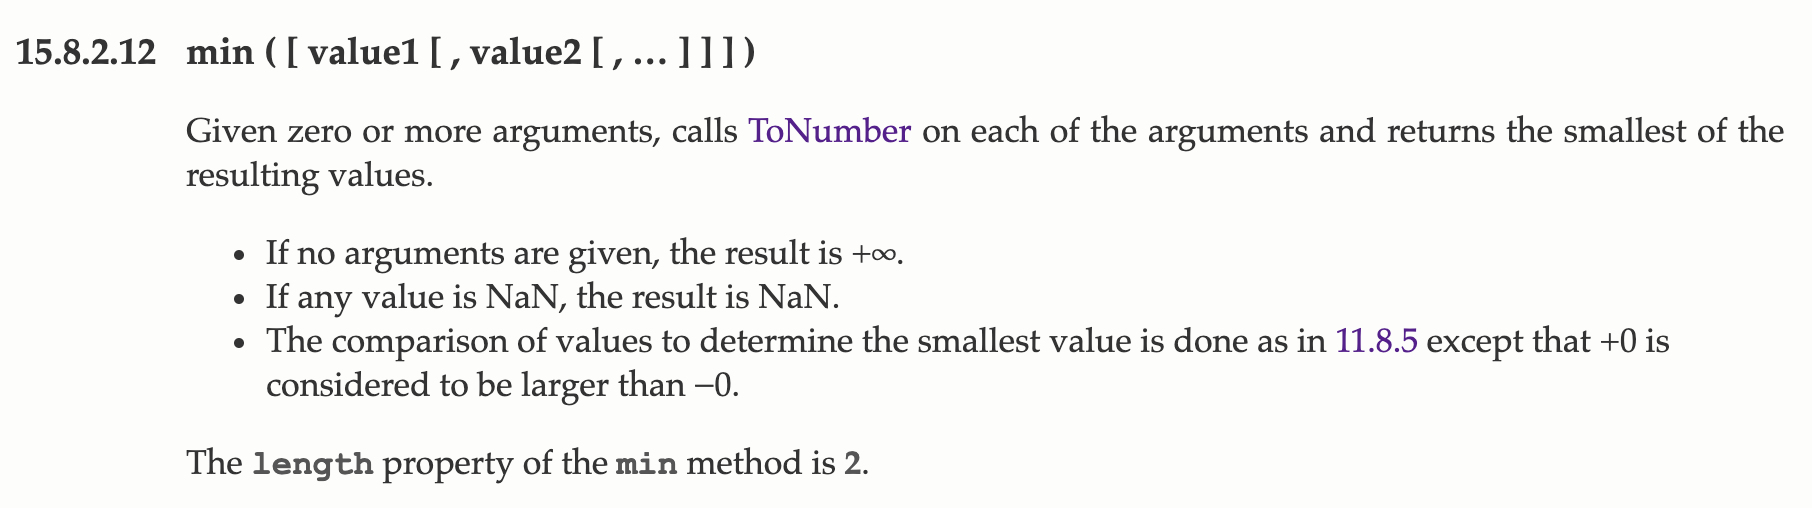
\includegraphics[width=1\textwidth]{figures/approach/type-inference/behavior_correctness/ecma-script-min-specification.png}}
		\caption[Math.min()]{\textbf{Math.min()} - Specification of the \mintinline{text}{Math.min()} method according to the ECMAScript Language Specification \citep{ecma-script}.}
		\label{fig:type-inference-ecma-script-min-specification}
	\end{centering}
\end{figure}

According to the specification of the native \mintinline{text}{Math.min()} method, each argument will be converted to a number before actually computing the minimum \citep{ecma-script}. Therefore, according to the definition shown in \figref{fig:type-inference-ecma-script-min-specification}, it is possible to compute the minimum between, for example, an \mintinline{text}{object} and a \mintinline{text}{function}. Although legal, there is no reasonable argument to define the examples in \coderef{code:type-inference-multiply-probably-incorrect} as correct.

\begin{code}
  \jscode{code/type-inference/definition-of-incorrect/math_min.js}
  \captionsetup{aboveskip=0pt, belowskip=10pt}
  \caption[Math.min() possible usage]{\textbf{Math.min() possible usage} - Invoking \mintinline{text}{Math.min()} with values of type different as \mintinline{text}{number} should not be expected.}
  \label{code:type-inference-multiply-probably-incorrect}
\end{code}

The key aspect is that the ECMAScript Language Specification defines behavior. It perfectly describes what is going to happen if a developer invokes \textit{Math.min()} with an argument that is not a \mintinline{text}{number}: every argument will be coerced to a \mintinline{text}{number}. However, such a definition is not related to \textit{correctness}.

Ryan Cavanaugh, development lead for the TypeScript team at Microsoft, stated the following\footnote{https://stackoverflow.com/questions/41750390/what-does-all-legal-javascript-is-legal-typescript-mean}:

\begin{displayquote}
  \textit{After all, this code does have defined behavior! But this misses the forest for the trees - it is plainly implausible that this code is correct for any reasonable definition of "correct". TypeScript's existence is predicated on the notion that some JavaScript code is not correct and you'd like to know about it.}
  \\
  \\
  \textit{The fact that the spec describes what happens is not instructive as to whether or not you're writing a correct program. A doctor can clearly describe what will happen to you if you eat a rock, but that doesn't mean rocks are food.}
\end{displayquote}

Probably no developer would argue with the fact that \mintinline{text}{Math.min()} should indeed receive numbers as arguments. Actually, TypeScript only accepts numbers as possible arguments for \mintinline{text}{Math.min()}, as shown in \

\begin{code}
  \tscode{code/type-inference/definition-of-incorrect/math_min_typescript_definition.ts}
  \captionsetup{aboveskip=0pt, belowskip=10pt}
  \caption[TypeScript definition for Math.min()]{\textbf{TypeScript definition for Math.min()} - TypeScript defines \mintinline{text}{Math.min()} as a function that receives arguments only of type \mintinline{text}{number}.}
  \label{code:type-inference-math-min-typescript-definition}
\end{code}

\subsection{Case study: inference for \mintinline{text}{+} operator}

The following section exposes the difficulties that may arise when trying to infer the type of a value using the \mintinline{text}{+} operator.

\coderef{code:type-inference-string-concatenation} provides an example where a function can be reasonably used with a \mintinline{text}{string}, a \mintinline{text}{number} or even an \mintinline{text}{object}. On the other hand, \coderef{code:type-inference-string-concatenation-only-string} presents an example using the same \mintinline{text}{+} operator where only a \mintinline{text}{string} would be accepted.

Finally, for both cases it would be technically correct to infer the input argument as \mintinline{text}{any}. JavaScript will accept a value of any type and will perform the according type coercion without throwing any run-time error. It is clear then that the developer's intention is the most relevant aspect for inferring a type.

\begin{code}
  \jscode{code/type-inference/example-plus-operator/string-concatenation.js}
  \captionsetup{aboveskip=0pt, belowskip=10pt}
  \caption[Operator + used with string and number]{\textbf{Operator + used with \mintinline{text}{string} and \mintinline{text}{number}} - The following simple function can be invoked with a \mintinline{text}{string}, a \mintinline{text}{number} or even an \mintinline{text}{object} with a defined \mintinline{text}{valueOf} method.}
  \label{code:type-inference-string-concatenation}
\end{code}

\begin{code}
  \jscode{code/type-inference/example-plus-operator/string-concatenation-only-string.js}
  \captionsetup{aboveskip=0pt, belowskip=10pt}
  \caption[Operator + used only with string]{\textbf{Operator + used with \mintinline{text}{string}} - The following function provides an example where only a \mintinline{text}{string} would be accepted.}
  \label{code:type-inference-string-concatenation-only-string}
\end{code}

\subsection{Constraints and restrictions}
The following section presents the restrictions that different type checkers perform on JavaScript code. The state of the art is shown through a comparison between \mintinline{text}{TypeScript}, \mintinline{text}{Flow} and \mintinline{text}{Infernu}. All of them introduce the concept of restrictions for JS from different angles and for different use cases. The analysis is going to be performed on the \mintinline{text}{+} operator.

\subsubsection{TypeScript}
Typescript defines the \mintinline{text}{+} operator using the table presented in \figref{fig:type-inference-typescript-definition-plus-operator}. It is important to note that TypeScript allows a \mintinline{text}{string} to be added to anything. On the other hand, it does not allow, for example, to add a \mintinline{text}{boolean} and an \mintinline{text}{object} or a \mintinline{text}{number} and a \mintinline{text}{boolean}.

\begin{figure}[tp]
	\centering
	\subfloat[Table with allowed types for the \mintinline{text}{+} operator]{
		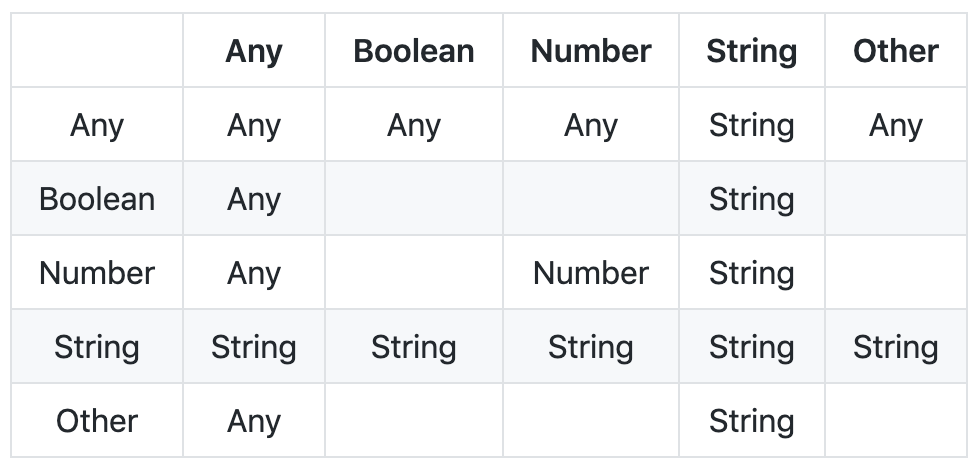
\includegraphics[width=0.6\textwidth]{figures/approach/type-inference/typescript_plus_operator.png}
	}

	\begin{lrbox}{\mintedbox}
		\begin{minipage}{0.7\textwidth}
			\tscode{code/type-inference/constraints/constraints-typescript.ts}
		\end{minipage}
	\end{lrbox}
	\subfloat[Examples of not allowed operations]{\usebox{\mintedbox}}

	\caption[TypeScript definition of the + operator]{\textbf{TypeScript definition of the \mintinline{text}{+} operator} - Rows and columns of the table represent the type of the operands. Values within the table represent the type of the return value. The empty cells specify the invalid operations.}
	\label{fig:type-inference-typescript-definition-plus-operator}
\end{figure}

\subsubsection{Flow}
Flow is a static type checker for JavaScript developed by Facebook \citep{flow}\citep{FLOW_DBLP:journals/pacmpl/ChaudhuriVGRL17}. It is intended to aid developers while writing JS code by detecting different errors. It only allows to use the \mintinline{text}{+} operator between \mintinline{text}{string} and \mintinline{text}{string}, \mintinline{text}{number} and \mintinline{text}{number} or \mintinline{text}{string} and \mintinline{text}{number}, as explained in \coderef{code:type-inference-constraints-flow}.

\begin{code}
  \jscode{code/type-inference/constraints/constraints-flow.js}
  \captionsetup{aboveskip=0pt, belowskip=10pt}
  \caption[Restrictions in Flow type checker]{\textbf{Restrictions in Flow type checker} - The \mintinline{text}{+} can be used only with \mintinline{text}{string} or \mintinline{text}{number}.}
  \label{code:type-inference-constraints-flow}
\end{code}


\subsubsection{Infernu}
Infernu is a static type checker for JavaScript that applies the concept of Type Classes to JS \citep{infernu}. It is inspired by Haskell's Type Classes. According to Infernu's documentation, operator \mintinline{text}{+} can be used only when both operands are either \mintinline{text}{string} or \mintinline{text}{number}, as shown in \coderef{code:type-inference-constraints-infernu}.

\begin{code}
  \jscode{code/type-inference/constraints/constraints-infernu.js}
  \captionsetup{aboveskip=0pt, belowskip=10pt}
  \caption[Restrictions in Infernu type checker]{\textbf{Restrictions in Infernu type checker} - The \mintinline{text}{+} can be used only when both operands are either \mintinline{text}{string} or \mintinline{text}{number}.}
  \label{code:type-inference-constraints-infernu}
\end{code}


\subsection{Proposal}
The challenge in type inference automation is to capture the developer's intention. It is fundamental to understand the code written by the developer. As explained, JavaScript is a language for which very unintuitive operations do not throw any errors at run-time. Developers may be already using this kind of behavior consciously by creating uncommon patterns which are useful in different scenarios. Therefore, working with constraints and hard rules that forbid certain operations, like adding an \mintinline{text}{array} and a \mintinline{text}{number}, is not ideal.

The proposal is to use a scoring system that favors coding best practices and disfavors uncommon or unexpected ones. In the end, based on this scoring you can infer the type of the variable, since types with higher score will represent the developer's intention more accurately. Uncommon operations will not be restricted but they would get lower scores. The scoring is generated by registering all interactions performed by the code to a particular variable.

Applying the presented approach would mean that despite uncommon usage of a particular type, if there is enough evidence that supports the developer's intention, that type should be inferred anyway.

\coderef{code:type-inference-unintuitive-developers-intention} presents a code where it is clear that \mintinline{text}{a} is an \mintinline{text}{array}. We see in line 9 that the developer is using an array with the \mintinline{text}{+} operator. It is known that such an usage is not common. However, there is enough evidence to support inferring \mintinline{text}{a} as an \mintinline{text}{array}. We are therefore assuming that the developer is consciously adding the number \mintinline{text}{1} to an \mintinline{text}{array}. In fact, applying a constraint on using an \mintinline{text}{array} with the \mintinline{text}{+} operator would have made it impossible to actually infer the type \mintinline{text}{array}.

\begin{code}
  \jscode{code/type-inference/proposal/intention-to-use-array.js}
  \captionsetup{aboveskip=0pt, belowskip=10pt}
  \caption[Unintuitive developer's intention]{\textbf{Unintuitive developer's intention} - The developer's intention of using \mintinline{text}{a} as an \mintinline{text}{array} is clear, despite the usage of the \mintinline{text}{+} operator. A scoring system would assign a high score to the type \mintinline{text}{array} because of other hints in the code and therefore the type of \mintinline{text}{a} would be inferred as \mintinline{text}{array}.}
  \label{code:type-inference-unintuitive-developers-intention}
\end{code}

Code examples provided by the developer should be considered as additional hints for inferring a type. In fact, they should be considered as very strong indicators, since the developer is explicitly stating her intention through code.

There is no doubt about the developer's intention, however, when an interface needs to be inferred. The developer explicitly reveals the shape of the required interface by accessing an object's property or invoking a method.

Finally, in order to define a scoring system it is crucial to understand what the developers are expecting from each operation and how are they using them. For answering those questions, it is necessary to analyze existing code bases and extracting common patterns. \secref{sec:experiments-js-operators-usage} presents the results from the analysis performed for this approach, where a heat map was created for each operator by analyzing existing JS libraries uploaded to the NPM registry. This way, the most common types for different operators could be identified. The following section discusses the application of the obtained results.

\subsubsection{Scoring for operators}
Results presented in \secref{sec:experiments-js-operators-usage} are briefly commented in the following section. Information was retrieved by execution JavaScript libraries through the code examples in the repositories, so the results intent to represent the developer's common usage. Obtained values are used to create a scoring for operators and the type of their operands. Analyze is limited to operators \mintinline{text}{+} and \mintinline{text}{===} but they can be easily extended. Usage distribution for these operators are presented in \figref{fig:type-inference-proposal-scoring-plus} and \figref{fig:type-inference-proposal-scoring-strict-equal}. Scores can be built using the results. For operator \mintinline{text}{+}, when an operand is known to be a \mintinline{text}{number}, the second operand is extremely likely to be also a \mintinline{text}{number} and should therefore be greatly favored.

\begin{figure}[tp]
	\centering
	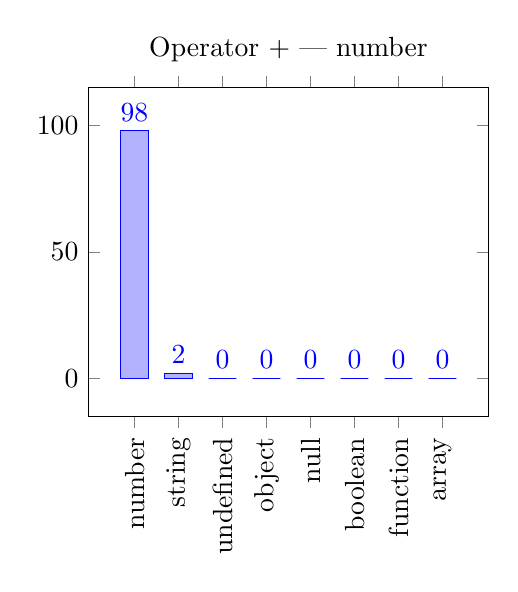
\begin{tikzpicture}
		\begin{axis}[
			ybar,
			title=Operator + | number,
			width=0.55\textwidth,
			ybar=0pt,
			ymax=100,
			enlargelimits=0.15,
			legend style={at={(0.5,-0.2)}, anchor=north,legend columns=-1},
			symbolic x coords={number,string,undefined,object,null,boolean,function,array},
			xtick=data,
			nodes near coords, 
			nodes near coords align={vertical},
			x tick label style={rotate=90,anchor=east},
		]
		\addplot coordinates {
			(number, 98)
			(string, 2)
			(undefined, 0)
			(object, 0)
			(null, 0)
			(boolean, 0)
			(function, 0)
			(array, 0)
		};
		\end{axis}
	\end{tikzpicture}
	%
	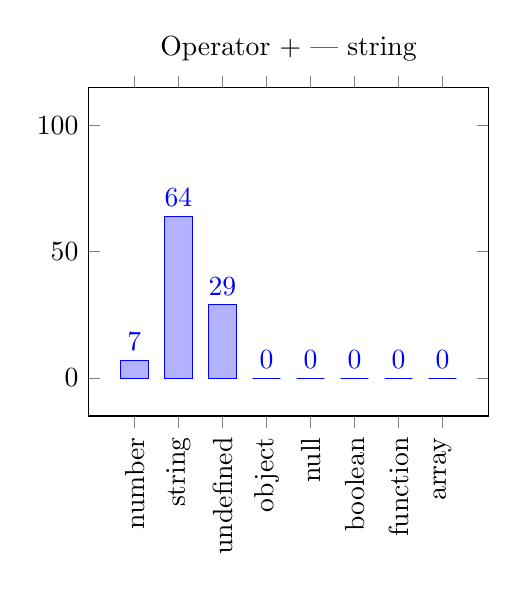
\begin{tikzpicture}
		\begin{axis}[
			ybar,
			title=Operator + | string,
			width=0.55\textwidth,
			ybar=0pt,
			ymax=100,
			enlargelimits=0.15,
			legend style={at={(0.5,-0.2)}, anchor=north,legend columns=-1},
			symbolic x coords={number,string,undefined,object,null,boolean,function,array},
			xtick=data,
			nodes near coords, 
			nodes near coords align={vertical},
			x tick label style={rotate=90,anchor=east},
		]
		\addplot coordinates {
			(number, 7)
			(string, 64)
			(undefined, 29)
			(object, 0)
			(null, 0)
			(boolean, 0)
			(function, 0)
			(array, 0)
		};
		\end{axis}
	\end{tikzpicture}

	\caption[Usage distribution for operator +]{\textbf{Usage distribution for operator \mintinline{text}{+}} - Both graphs were made by fixing the type of one of the operands. If a value is used with the operator \mintinline{text}{+} and the other operand is a \mintinline{text}{number}, the graph on the left should be used. If the second operand is a \mintinline{text}{string}, the graph on the right should be used.
	}

	\label{fig:type-inference-proposal-scoring-plus}
\end{figure}

\begin{figure}[tp]
	\centering
	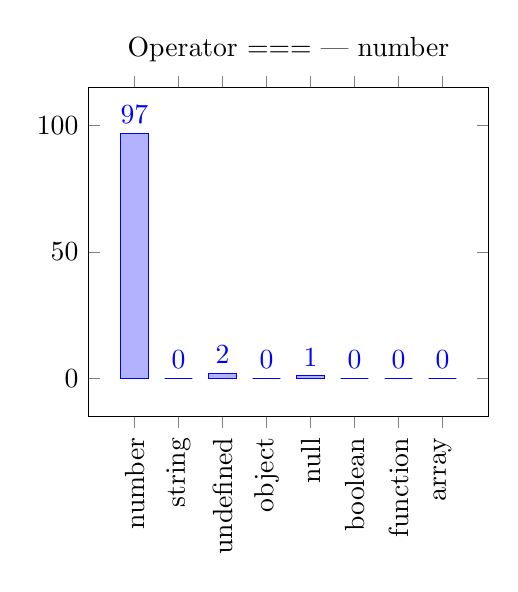
\begin{tikzpicture}
		\begin{axis}[
			ybar,
			title=Operator ${===}$ | number,
			width=0.55\textwidth,
			ybar=0pt,
			ymax=100,
			enlargelimits=0.15,
			legend style={at={(0.5,-0.2)}, anchor=north,legend columns=-1},
			symbolic x coords={number,string,undefined,object,null,boolean,function,array},
			xtick=data,
			nodes near coords, 
			nodes near coords align={vertical},
			x tick label style={rotate=90,anchor=east},
		]
		\addplot coordinates {
			(number, 97)
			(string, 0)
			(undefined, 2)
			(object, 0)
			(null, 1)
			(boolean, 0)
			(function, 0)
			(array, 0)
		};
		\end{axis}
	\end{tikzpicture}
	%
	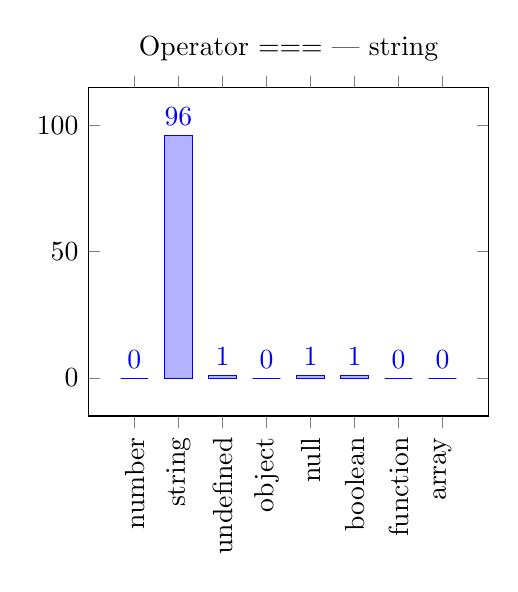
\begin{tikzpicture}
		\begin{axis}[
			ybar,
			title=Operator ${===}$ | string,
			width=0.55\textwidth,
			ybar=0pt,
			ymax=100,
			enlargelimits=0.15,
			legend style={at={(0.5,-0.2)}, anchor=north,legend columns=-1},
			symbolic x coords={number,string,undefined,object,null,boolean,function,array},
			xtick=data,
			nodes near coords, 
			nodes near coords align={vertical},
			x tick label style={rotate=90,anchor=east},
		]
		\addplot coordinates {
			(number, 0)
			(string, 96)
			(undefined, 1)
			(object, 0)
			(null, 1)
			(boolean, 1)
			(function, 0)
			(array, 0)
		};
		\end{axis}
	\end{tikzpicture}
	%
	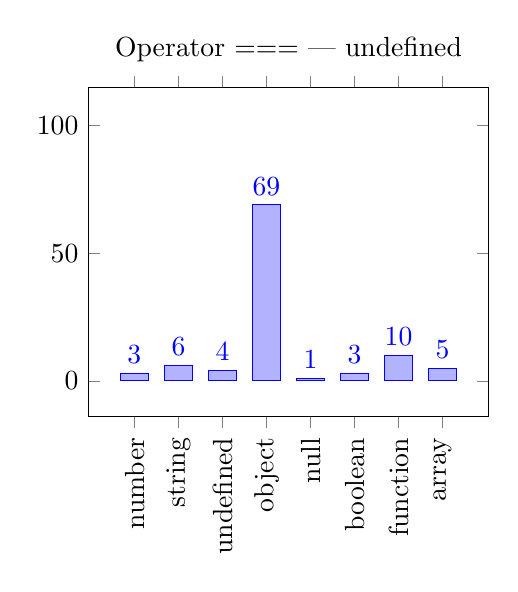
\begin{tikzpicture}
		\begin{axis}[
			ybar,
			title=Operator ${===}$ | undefined,
			width=0.55\textwidth,
			ybar=0pt,
			ymax=100,
			enlargelimits=0.15,
			legend style={at={(0.5,-0.2)}, anchor=north,legend columns=-1},
			symbolic x coords={number,string,undefined,object,null,boolean,function,array},
			xtick=data,
			nodes near coords, 
			nodes near coords align={vertical},
			x tick label style={rotate=90,anchor=east},
		]
		\addplot coordinates {
			(number, 3)
			(string, 6)
			(undefined, 4)
			(object, 69)
			(null, 1)
			(boolean, 3)
			(function, 10)
			(array, 5)
		};
		\end{axis}
	\end{tikzpicture}
	%
	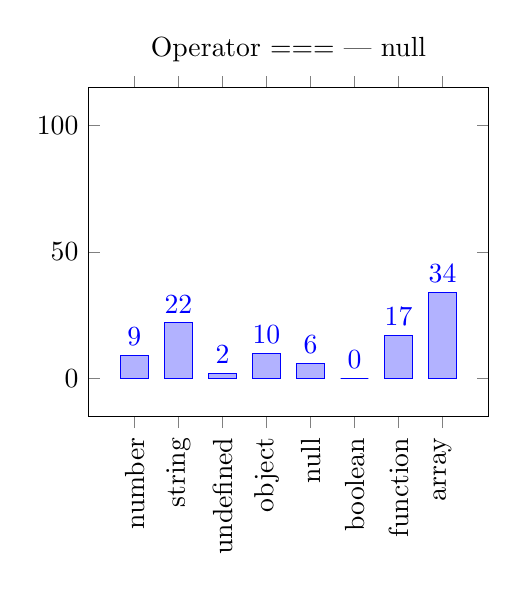
\begin{tikzpicture}
		\begin{axis}[
			ybar,
			title=Operator ${===}$ | null,
			width=0.55\textwidth,
			ybar=0pt,
			ymax=100,
			enlargelimits=0.15,
			legend style={at={(0.5,-0.2)}, anchor=north,legend columns=-1},
			symbolic x coords={number,string,undefined,object,null,boolean,function,array},
			xtick=data,
			nodes near coords, 
			nodes near coords align={vertical},
			x tick label style={rotate=90,anchor=east},
		]
		\addplot coordinates {
			(number, 9)
			(string, 22)
			(undefined, 2)
			(object, 10)
			(null, 6)
			(boolean, 0)
			(function, 17)
			(array, 34)
		};
		\end{axis}
	\end{tikzpicture}

	\caption[Usage distribution for operator ===]{\textbf{Usage distribution for operator \mintinline{text}{===}} - All graphs were made by fixing the type of one of the operands. That means, for example, that if a value is used with the operator \mintinline{text}{===} and the other operand is a \mintinline{text}{number}, the top-left graph should be used.}
	\label{fig:type-inference-proposal-scoring-strict-equal}
\end{figure}
